\documentclass[10pt,twocolumn,letterpaper]{article}

\usepackage{cvpr}
\usepackage{times}
\usepackage{epsfig}
\usepackage{graphicx}
\usepackage{amsmath}
\usepackage{amssymb}





% Include other packages here, before hyperref.

% If you comment hyperref and then uncomment it, you should delete
% egpaper.aux before re-running latex.  (Or just hit 'q' on the first latex
% run, let it finish, and you should be clear).
\usepackage[breaklinks=true,bookmarks=false]{hyperref}

\usepackage{siunitx}
\usepackage{amssymb}

\usepackage[breaklinks=true,bookmarks=false]{hyperref}
\usepackage{listings}
\usepackage{graphicx}
\usepackage{caption2}
\usepackage{subfigure}
\usepackage{float}

\cvprfinalcopy % *** Uncomment this line for the final submission

\def\cvprPaperID{****} % *** Enter the CVPR Paper ID here
\def\httilde{\mbox{\tt\raisebox{-.5ex}{\symbol{126}}}}

% Pages are numbered in submission mode, and unnumbered in camera-ready
%\ifcvprfinal\pagestyle{empty}\fi
\setcounter{page}{1}
\begin{document}

%%%%%%%%% TITLE
\title{CS181 Artificial Intelligence I: \\ Final Project : A Minesweeper Using Inference, CSP and CNN}

\author{Chenyang Zhang, Chunxu Guo, Jiahao Huang, Qianyu Liu, Tianyi Zhang\\

%Institution1\\
%Institution1 address\\
{\tt\small .@shanghaitech.edu.cn}
% For a paper whose authors are all at the same institution,
% omit the following lines up until the closing ``}''.
% Additional authors and addresses can be added with ``\and'',
% just like the second author.
% To save space, use either the email address or home page, not both
%\and
%Second Author\\
%Institution2\\
%First line of institution2 address\\
%{\tt\small secondauthor@i2.org}
}

\maketitle
%\thispagestyle{empty}

%%%%%%%%% ABSTRACT
\begin{abstract}
Minesweeper is a single-player puzzle computer video game written by Robert Donner ami Curt Johnson which include in Microsoft Windows$^{\copyright}$ in 1991, whose goal is to clear a rectangular board containing hidden 'mines' or bombs without detonating any of them. This game originates from 1960s and has derived different variants on many computing platforms. In fact, Minesweeper is proved to be Turning Complete and in a class of mathematically difficult problems known as co-NP-complete as well. Exploring algorithms to solve Minesweeper game may inspire us to work out other related problems.
\end{abstract}


%%%%%%%%% BODY TEXT
\section{Introduction}
Minesweeper game is basically defined in a custom-sized square grid board with a certain number of mined. The most classical and standard size of mine board is 9$\times$9 (beginner),  16$\times$16 (intermediate), 16$\times$30 (advanced), and the standard mine density of advanced one is 20.63%.(Usually mine density will be higher than this ratio.) 

There are 2 main competitive direction for Minesweeper players, one is speed and the other one is correctness. Algorithm model in this report is tend to revealing safe cells as much as possible without limited time. As it is proved to be an NP-hard problem in 2000, no such algorithm could solve it in linear time complexity so far. Besides, Minesweeper game might sometimes become a non-deterministic problem, which is roughly regarded as a classical models of probability now.(Suppose that all the mine matrices are randomly  generated in the beginning, satisfying the uniform distribution.) Under this circumstance, neither people and computer could definitely reveal a risk-free cell. 

Playing Minesweeper game requires logic, arithmetic and probabilistic reasoning knowledge based on spatial relationships on the mine board. Up to now, multiple artificial Intelligent algorithms have been proposed to solve minesweeper game, such as Inference, Constraint Satisfaction Problem (CSP) with backtracking, Markov Decision Process (MDP) or Partially Observable Markov Decision Process (POMDP), SAT solver, neural network and so on. Considering their performance as well as related with course CS181, we design an identical algorithm model combining logic, CSP and convolution neural network (CNN). The most complicated case among our test condition 16$\times$30 with 20.83\% mine ratio. 


\section{Related works}
\textcolor{red}{pass}


\section{Basic Idea for Minesweeper}

In a Minesweeper game, players will be given a certain sized grid board and the number M of unknown mines.  Initially, all the sub-squares or the cells are blank, hidden among them are M mines distributed uniformly at random.  To clarify the subsequent description, we raise some useful concepts here.
	\begin{itemize}
		\item \textbf{Neighbors}: unrevealed one in 8 surrounding blocks are all the neighbors of a given block.
		\item \textbf{Set} : A group of unmarked neighbors around a certain number block.
		\item \textbf{Game Map} : Real world interaction graph, a visual mine board with cells blank or filled with integer n. n varies from 0 to 8.
		\item \textbf{Mine Map} : Grand truth, the real mine distribution that we do not know.
		\item \textbf{Cell State} : At the beginning of game, all cells are signed with a initial state as {1,0}, which means not sure about whether a cell has a mine. If a cell has been inferred as safe definitely, update the cell state as {0}. Else if a cell has been inferred with mine definitely, update the cell state as {1}. Otherwise stick to the original cell state.
		\item \textbf{Transfered Map} : A local graph used in CSP phase, each cell in this graph are related to a cell state.
		\item \textbf{Turn} : Every time the player operates once is a turn.
	\end{itemize}
	
At each turn, a real world player can select three possible actions: to flag a cell as mine, to unmark a flagged cell, and to reveal a cell. But for AI robots, it would only maintain the transformed map corresponding to game map and click on safe cell with cell state = {0}, unless no such cell is definitely safe. Under that uncertain circumstance, clicking depends on the descending order of global probability.

By clicking, player will safely reward a number behind(sometimes a large area will also be revealed fortunately) or lose the game immediately after detonating a mine. Until all the safe cells are revealed our lucky player wins. 



\section{Our Strategy}
The main pipeline of our algorithm model in this report is shown below (Figure 1), involving junior and senior logic reasoning method and probalistic calculation.
     \begin{figure}[H]
     \centering
     \subfigure[Figure 1]{
     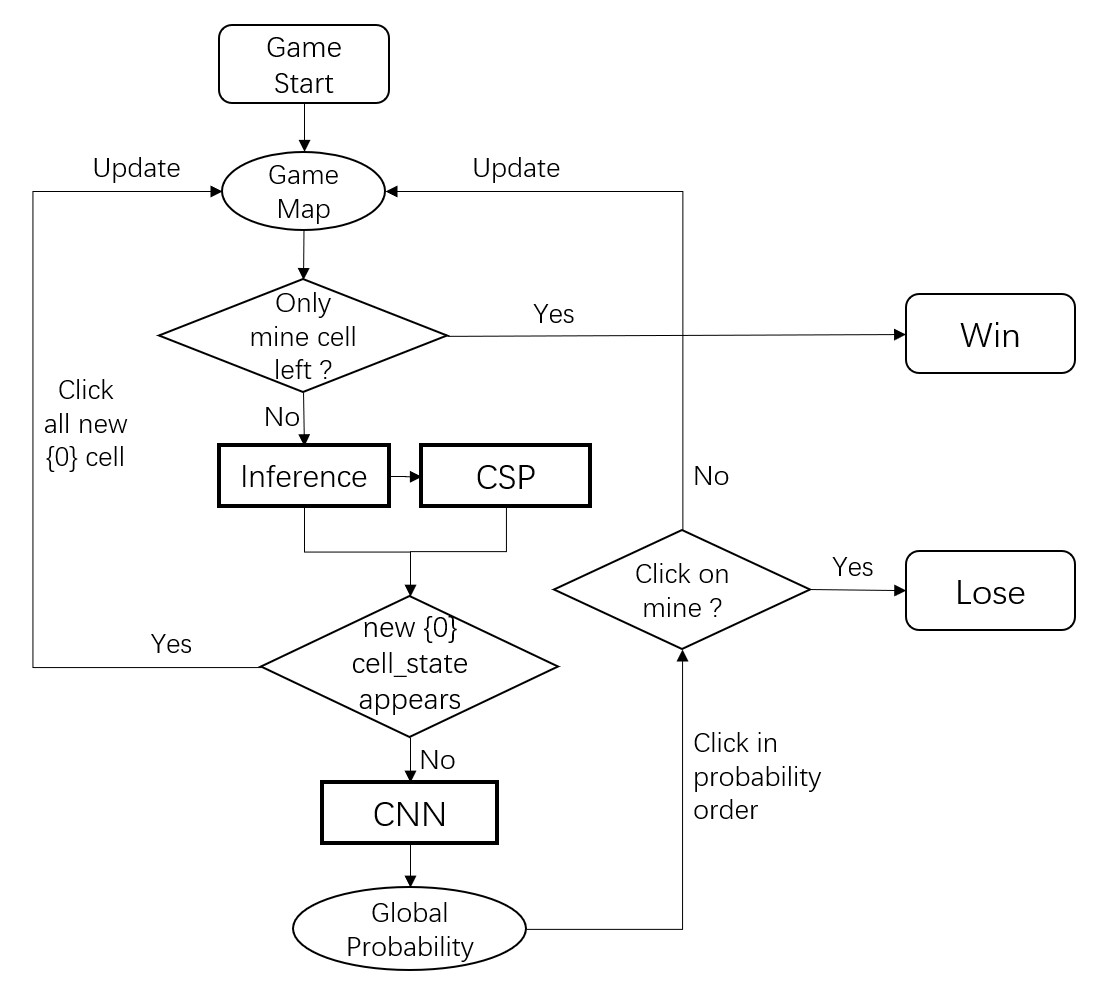
\includegraphics[width=0.5\textwidth]{import_pic//workflow.jpg} 
 }
     \label{workflow}
     \end{figure}
      
Junior logic reasoning, the fastest and simplest cell assignment stage in our model, which is placed at the most front, only uses the adjacent 3$\times$3 patches' constaints to figure out deterministic safe and mine-behind cells. Over half of situation could be solved after this stage. While sometimes it is not enough only considering adjacent information, so that a senior logic reasoning method called CSP followed. The magic power of CSP is embodied in cell constaint merge and division. In other words it create some new constraints on nonfixed shaped patches, and advancedly compare all the patch pairs instaead of adjacent ones. The complexity of this method grows almost as exponential as the scale of the mine board due to the rapid increase of constaints space. Backtracking may help us pruning a lot but it is still much slower than simple inference. CSP is also used to figure out deterministic safe and mine-behind cells.

Either after Inference or CSP stage, if AI robot could click on some safe cells, Game Map and Transfered Map will be miantained and reveal some new mine information which could be used for constraint update. Inference and CSP are able to run as far as possible with such regenerative feedback. Unavoidably, sometimes mine situation will fall into a 'dead corner' and bring about a 'guess' turn. None of the remaining unclicked cells can be definitely assigned with a deterministic state, and the only choice left is to click on the most likely cells without mines. CNN, the last module of our workflow in Figure 1 helps us to build a global probability table. Fine grid kernel helps to worked out neighbors contribution, while the coarse grid kernel provides a greater field of reception, combination of two of them enables local constraint relationships to transform into global probabilities.


\subsection{Inference}
Inference is the most basic step in our algorithm applying 4 basic rules as followed:
	\begin{itemize}
		\item Theorem 1 : If \#(items) in set is equal to number on block minus mine neighbours,then all the blocks in set can be marked as mines
		\item Theorem 2 : For 2 number blocks \textbf{a} and \textbf{b}, suppose \textbf{A} and \textbf{B} are their corresponding block set, if \textbf{A} $\subseteq$ \textbf{B} and number on \textbf{a} minus \#(marked neighbours) is equal to number on \textbf{b} minus \#(marked neighbours), then blocks in complement of \textbf{A} refer to \textbf{B} can be all revealed safely.
		\item \textcolor{red}{eliminate}
		\item \textcolor{red}{confirm}
	\end{itemize}
	 


\subsection{Constraint Satisfaction Problem (CSP) with backtracking}
\textcolor{red}{pass}

\subsection{Convolutional Neural Networks (CNN)}
\textcolor{red}{pass}

\section{Experiment and Result}
     \begin{figure}[H]
     \centering
     \subfigure[Figure 2]{
     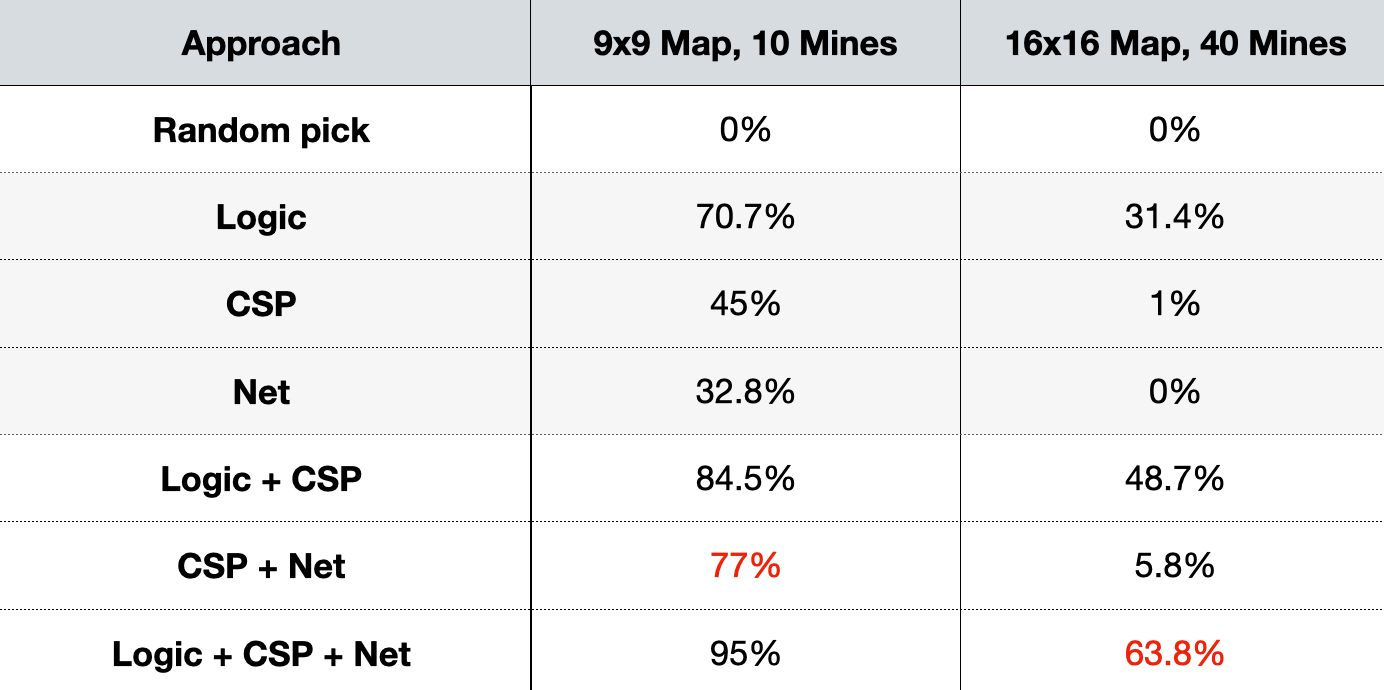
\includegraphics[width=0.45\textwidth]{import_pic//result.png} 
 }
     \label{result}
     \end{figure}

\section{Discussion}



{\small
\bibliographystyle{ieee_fullname}
\bibliography{egbib}
}

\end{document}
